\section{ModuleDG}
%\justifying

\subsection{Définition}
\paragraph{}
ModuleDG est un web service développé par Data-Gest qui sert à :
\begin{itemize}
\item [-] Gestion des commandes envoyé depuis chaque site.
\item [-] Gestion de la sélection de cadeaux de chaque site.(incentive/kdomotive et Clubdotations)
\item [-] Gestion du catalogue (Base cadeau et les vitrines communes)
\item [-] L’intégralité des commandes enregistrées (si une commande est supprimer à cet endroit cela met à jour le site de l’opération concernée et re-crédite de façon mécanique les points correspondant à la somme de la valeur des articles\end{itemize}


\subsection{Structure}
\paragraph{}
La fonctionnalité est bien illustré dans le figure suivant.


\begin{figure}[hbtp]
\center
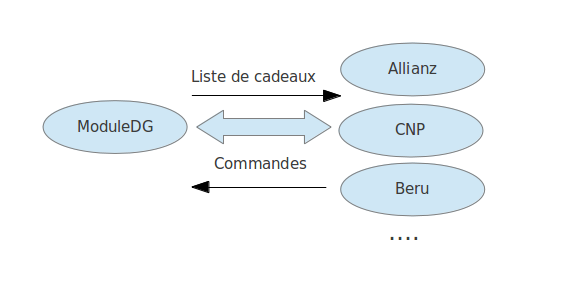
\includegraphics[width=15cm]{body/images/ModuleDG.png}
\caption{Structure de ModuleDG}
\end{figure}



\paragraph{}
En fait chaque site a une sélection de cadeaux qui est géré par  ModuleDG. Quand le client de chaque site valide une commande, il sera passé à moduleDG afin de contrôler.(Valider les commandes et les envoyer à expédition) 

La fonctionnalité entre ModuleDG est toujours comme ça.


